\documentclass{article}

\usepackage[margin=1in]{geometry}
\usepackage{graphicx} % Allow image/pdf includes
\usepackage{extramarks} % Extra header marks (continued on next page)
\usepackage{amsmath} % Math enhancements
\usepackage{amsthm} % Theorem typesetting
\usepackage{amssymb} % Extended symbol collection
\usepackage{tikz} % Graphical element creation
\usetikzlibrary{automata,positioning}
\usepackage{algpseudocode} % Algorithm layout
\usepackage{enumitem} % Enumerate (lists)
\usepackage{ragged2e} % Alternative alignment
\usepackage{gensymb} % Generic symbols (degree, etc)
\usepackage{empheq} % Allow \boxed around \begin{empheq}
\usepackage{color,soul} % Highlighting
\usepackage{booktabs} % Enhanced table creation
\usepackage{multirow} % Table multi row
\usepackage{mathtools} % Math enhancements
\usepackage{bm} % Bold math
\usepackage[mathscr]{euscript} % Script variables
\usepackage{cancel} % Cancel through text
\usepackage{color,soul} % Highlighting
\usepackage{mathtools}
\usepackage{multirow}
\usepackage{mathrsfs}
\usepackage{physics}
\usepackage{gensymb}
\usepackage{siunitx}
\usepackage{subcaption}
\usepackage[]{algorithm2e}
\usepackage{float}
\usepackage[cache=false]{minted}
\renewcommand{\MintedPygmentize}{/Users/loganharbour/miniconda/bin/pygmentize}
\usepackage[scaled]{beramono}
\usepackage[T1]{fontenc}
\usepackage{diagbox}

\setlength\parindent{0pt} % No indents
\setlength{\parskip}{1em} % Paragraph skip

\newcommand{\vx}{\mathbf{x}} % x vector
\newcommand{\vy}{\mathbf{y}} % x vector

\newcommand{\pageTitle}{MEEN 644 - Homework 4}
\newcommand{\pageAuthor}{Logan Harbour}

\begin{document}

\title{\LARGE \textbf{\pageTitle} \vspace{-0.3cm}}
\author{\large \pageAuthor}
\date{\vspace{-0.6cm} \large \today \vspace{-0.4cm}}

\maketitle

\section{Problem statement}

\begin{center}
	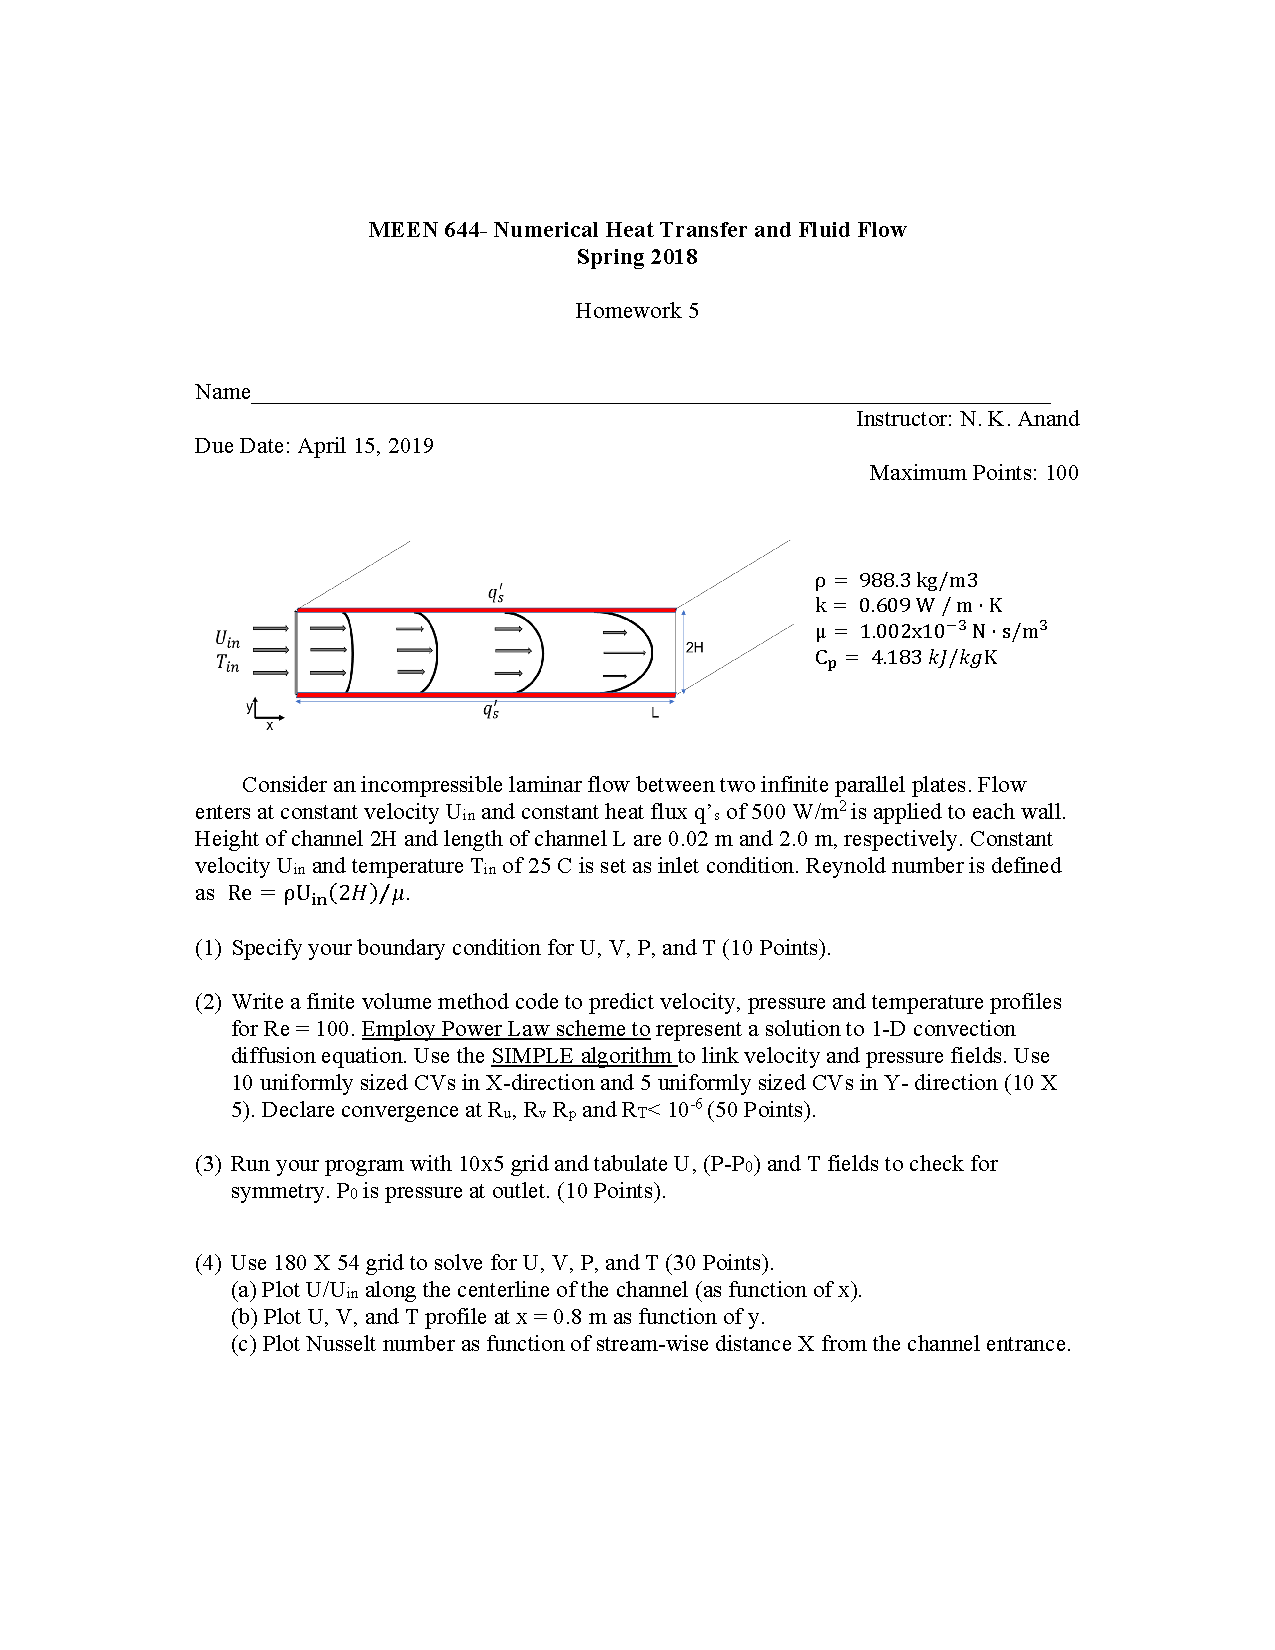
\includegraphics[trim={3.6cm 15.5cm 4cm 9.0cm},clip,page=1,scale=0.8]{../doc/hwk5.pdf}
\end{center}

Consider an incompressible laminar flow between two infinite parallel plates. Flow enters at constant velocity $u_\mathrm{in}$ and aconstant heat flux, $q' = 500$ W/m$^2$ is applied to each wall. Height of channel $2H$ and length of channel $L$ are 0.02 m and 2.0 m, respectively. Constant velocity $u_\mathrm{in}$ and temperature $T_\mathrm{in} = 25^\circ$C is set as the inlet condition. Reynolds number is defined as $Re = 2 \rho u_\mathrm{in} H / \mu$.
\begin{enumerate}
	\item \textbf{(10 points)} Specify your boundary condition for $u, v, P,$ and $T$.
	\item \textbf{(50 points)} Write a finite volume method code to predict velocity, pressure, and temperature profiles for Re = 100. Employ the Power Law scheme to represent a solution to a 1-D convection-diffusion equation. Use the SIMPLE algorithm to link velocity and pressure fields. Use 10 uniformly sized CVs in the $x$-direction and 5 uniformly sized CVs in the $y$-direction. Declare convergence at $R_u, R_v, R_P$ and $R_T < 10^{-6}$. 
	\item \textbf{(10 points)} Run your program with the 10 $\times$ 5 grid and tabulate $u, (P - P_0)$, and $T$ to check for symmetry. $P_0$ is the pressure at the outlet.
	\item \textbf{(30 points)} Use a $180 \times 54$ grid to solve for $u, v, P,$ and $T$.
	\begin{enumerate}[label=(\alph*)]
		\item Plot $u/u_\mathrm{in}$ along the centerline of the channel (as a function of $x$).
		\item Plot $u, v,$ and $T$ at $x = 0.8$m m (as a function of $y$).
		\item Plot the Nusselt number as a function of stream-wise distance $x$ from the channel entrance.
	\end{enumerate}
\end{enumerate}

\section{Preliminaries}

\subsection{Two-dimensional diffusion-convection}

\subsection{Solving methodology}

\subsection{Domain discretization}

The domain of size $L_x \times L_y$ is discretized into $N_x \times N_y$ uniformly sized control volumes with $\Delta x = L_x / N_x$ and $\Delta y = L_y / N_y$. The numbering for all variables begins at the origin at $(i, j) = (0, 0)$. The maximum index for each variable, $\phi$, is defined as $(M_x^\phi, M_y^\phi)$.

\section{Results}

\subsection{Problem 3: 10 $\times$ 5 grid}

The results requested for problem 3 follow in Tables \ref{table:coarse-u}, \ref{table:coarse-p-p0}, and \ref{table:coarse-T}.

\def\arraystretch{1.3}
\begin{table}[H]
	\scriptsize
	\centering
	\caption{The $u$-velocity solution with the 10 $\times$ 5 grid. A row corresponds to a $x$-position and a column corresponds to an $y$-position.}
	\vspace{0.2cm}
	\sisetup{output-exponent-marker = \text{E}, table-format=2.5e1,group-digits=false,retain-zero-exponent=true}
	\begin{tabular}{c|S|S|S|S|S|S|S}
		& {1} & {2} & {3} & {4} & {5} & {6} & {7} \\
		\hline
		1 & 2.50927e-03 & 2.50927e-03 & 2.50927e-03 & 2.50927e-03 & 2.50927e-03 & 2.50927e-03 & 2.50927e-03 \\
		2 & 0.00000e+00 & 1.44730e-03 & 3.04425e-03 & 3.56324e-03 & 3.04425e-03 & 1.44730e-03 & 0.00000e+00 \\
		3 & 0.00000e+00 & 1.39756e-03 & 3.06604e-03 & 3.61913e-03 & 3.06604e-03 & 1.39756e-03 & 0.00000e+00 \\
		4 & 0.00000e+00 & 1.39429e-03 & 3.06686e-03 & 3.62401e-03 & 3.06686e-03 & 1.39429e-03 & 0.00000e+00 \\
		5 & 0.00000e+00 & 1.39406e-03 & 3.06688e-03 & 3.62445e-03 & 3.06688e-03 & 1.39406e-03 & 0.00000e+00 \\
		6 & 0.00000e+00 & 1.39404e-03 & 3.06688e-03 & 3.62449e-03 & 3.06688e-03 & 1.39404e-03 & 0.00000e+00 \\
		7 & 0.00000e+00 & 1.39404e-03 & 3.06688e-03 & 3.62449e-03 & 3.06688e-03 & 1.39404e-03 & 0.00000e+00 \\
		8 & 0.00000e+00 & 1.39404e-03 & 3.06688e-03 & 3.62449e-03 & 3.06688e-03 & 1.39404e-03 & 0.00000e+00 \\
		9 & 0.00000e+00 & 1.39404e-03 & 3.06688e-03 & 3.62449e-03 & 3.06688e-03 & 1.39404e-03 & 0.00000e+00 \\
		10 & 0.00000e+00 & 1.39404e-03 & 3.06688e-03 & 3.62449e-03 & 3.06688e-03 & 1.39404e-03 & 0.00000e+00 \\
		11 & 0.00000e+00 & 1.39404e-03 & 3.06688e-03 & 3.62449e-03 & 3.06688e-03 & 1.39404e-03 & 0.00000e+00 \\
	\end{tabular}
	\label{table:coarse-u}
\end{table}

\def\arraystretch{1.3}
\begin{table}[H]
	\scriptsize
	\centering
	\caption{The $(P - P_0)$ solution with the 10 $\times$ 5 grid. A row corresponds to a $x$-position and a column corresponds to an $y$-position.}
	\vspace{0.2cm}
	\sisetup{output-exponent-marker = \text{E}, table-format=2.5e1,group-digits=false,retain-zero-exponent=true}
	\begin{tabular}{c|S|S|S|S|S|S|S}
		& {1} & {2} & {3} & {4} & {5} & {6} & {7} \\
		\hline
		1 & 1.41200e-01 & 1.41200e-01 & 1.41190e-01 & 1.41187e-01 & 1.41190e-01 & 1.41200e-01 & 1.41200e-01 \\
		2 & 1.41200e-01 & 1.41200e-01 & 1.41190e-01 & 1.41187e-01 & 1.41190e-01 & 1.41200e-01 & 1.41200e-01 \\
		3 & 1.18832e-01 & 1.18832e-01 & 1.18832e-01 & 1.18833e-01 & 1.18832e-01 & 1.18832e-01 & 1.18832e-01 \\
		4 & 1.04769e-01 & 1.04769e-01 & 1.04769e-01 & 1.04769e-01 & 1.04769e-01 & 1.04769e-01 & 1.04769e-01 \\
		5 & 9.07942e-02 & 9.07942e-02 & 9.07942e-02 & 9.07942e-02 & 9.07942e-02 & 9.07942e-02 & 9.07942e-02 \\
		6 & 7.68254e-02 & 7.68254e-02 & 7.68254e-02 & 7.68254e-02 & 7.68254e-02 & 7.68254e-02 & 7.68254e-02 \\
		7 & 6.28571e-02 & 6.28571e-02 & 6.28571e-02 & 6.28571e-02 & 6.28571e-02 & 6.28571e-02 & 6.28571e-02 \\
		8 & 4.88889e-02 & 4.88889e-02 & 4.88889e-02 & 4.88889e-02 & 4.88889e-02 & 4.88889e-02 & 4.88889e-02 \\
		9 & 3.49206e-02 & 3.49206e-02 & 3.49206e-02 & 3.49206e-02 & 3.49206e-02 & 3.49206e-02 & 3.49206e-02 \\
		10 & 2.09524e-02 & 2.09524e-02 & 2.09524e-02 & 2.09524e-02 & 2.09524e-02 & 2.09524e-02 & 2.09524e-02 \\
		11 & 0.00000e+00 & 0.00000e+00 & 0.00000e+00 & 0.00000e+00 & 0.00000e+00 & 0.00000e+00 & 0.00000e+00 \\
		12 & 0.00000e+00 & 0.00000e+00 & 0.00000e+00 & 0.00000e+00 & 0.00000e+00 & 0.00000e+00 & 0.00000e+00 \\
	\end{tabular}
	\label{table:coarse-p-p0}
\end{table}

\def\arraystretch{1.3}
\begin{table}[H]
	\scriptsize
	\centering
	\caption{The $T$ solution with the 10 $\times$ 5 grid. A row corresponds to a $x$-position and a column corresponds to an $y$-position.}
	\vspace{0.2cm}
	\sisetup{table-format=2.5,group-digits=false}
	\begin{tabular}{c|S|S|S|S|S|S|S}
		& {1} & {2} & {3} & {4} & {5} & {6} & {7} \\
		\hline
			1 & 26.64204 & 25.00000 & 25.00000 & 25.00000 & 25.00000 & 25.00000 & 26.64204 \\
			2 & 28.47372 & 26.83169 & 25.80190 & 25.50210 & 25.80190 & 26.83169 & 28.47372 \\
			3 & 30.21235 & 28.57032 & 26.64040 & 26.07996 & 26.64040 & 28.57032 & 30.21235 \\
			4 & 31.50432 & 29.86229 & 27.56664 & 26.82629 & 27.56664 & 29.86229 & 31.50432 \\
			5 & 32.60351 & 30.96148 & 28.51796 & 27.67470 & 28.51796 & 30.96148 & 32.60351 \\
			6 & 33.62161 & 31.97957 & 29.47406 & 28.57704 & 29.47406 & 31.97957 & 33.62161 \\
			7 & 34.60455 & 32.96252 & 30.43017 & 29.50634 & 30.43017 & 32.96252 & 34.60455 \\
			8 & 35.57185 & 33.92982 & 31.38560 & 30.44874 & 31.38560 & 33.92982 & 35.57185 \\
			9 & 36.53202 & 34.88999 & 32.34047 & 31.39739 & 32.34047 & 34.88999 & 36.53202 \\
			10 & 37.48883 & 35.84679 & 33.29498 & 32.34898 & 33.29498 & 35.84679 & 37.48883 \\
			11 & 38.44391 & 36.80187 & 34.24921 & 33.30189 & 34.24921 & 36.80187 & 38.44391 \\
			12 & 39.39900 & 37.75696 & 35.20344 & 34.25481 & 35.20344 & 37.75696 & 39.39900 \\
	\end{tabular}
	\label{table:coarse-T}
\end{table}

\subsection{Problem 4: 180 $\times$ 54 grid}

The requirements for problem (b) part i and ii were combined into Figure \ref{fig:p2} as seen below. With increasing grid refinement, both centerline velocity profiles approached towards the reference solution obtained from Roy et. al. In addition, a once-more-refined run is compared with 256x256 CVs with good agreement.

\begin{figure}[H]
	\centering
	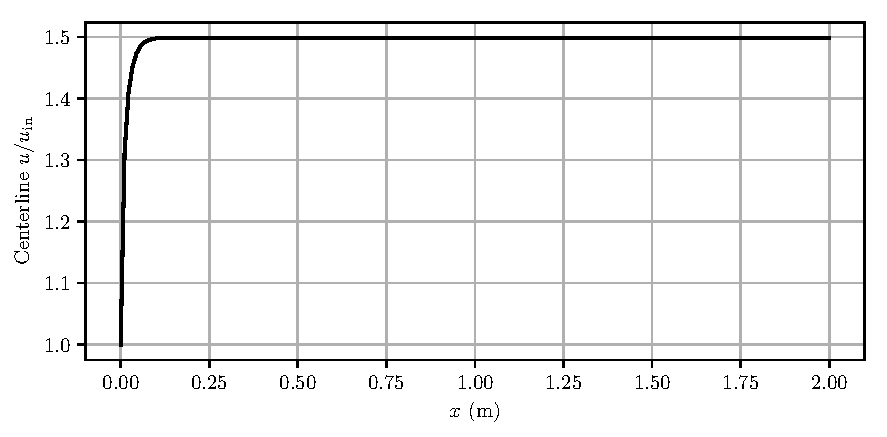
\includegraphics[width=0.75\linewidth]{../results/u_centerline}
	\caption{$u/u_\mathrm{in}$ plotted along the centerline of the channel for the 180 $\times$ 54 grid.}
	\label{fig:u-centerline}
\end{figure}

\begin{figure}[H]
	\centering
	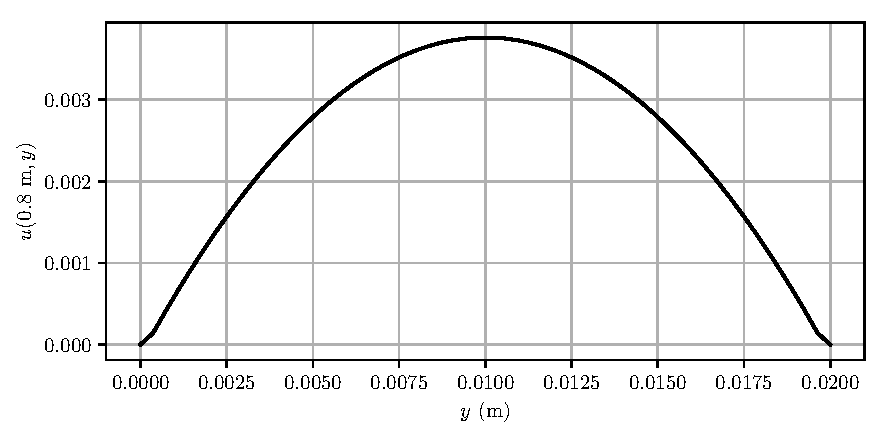
\includegraphics[width=0.75\linewidth]{../results/u_0p8}
	\caption{$u$ plotted at $x = 0.8$ m for the 180 $\times$ 54 grid.}
	\label{fig:u-0p8}
\end{figure}

\begin{figure}[H]
	\centering
	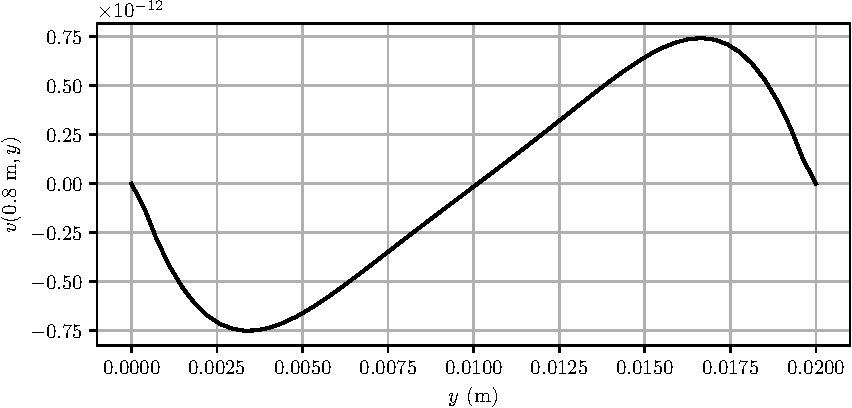
\includegraphics[width=0.75\linewidth]{../results/v_0p8}
	\caption{$v$ plotted at $x = 0.8$ m for the 180 $\times$ 54 grid.}
	\label{fig:v-0p8}
\end{figure}

\begin{figure}[H]
	\centering
	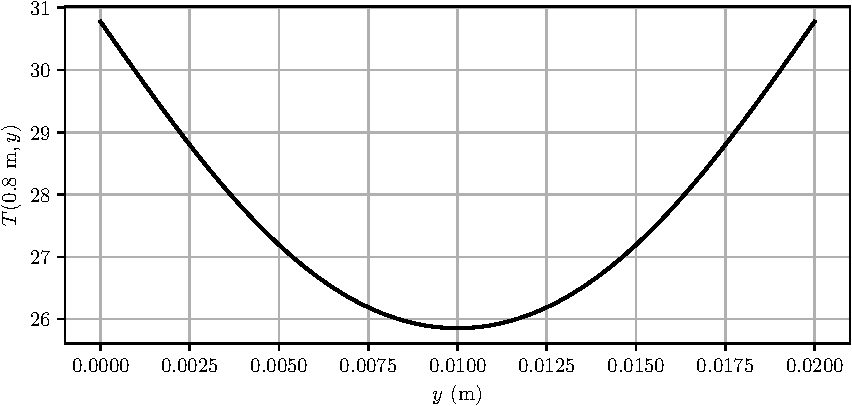
\includegraphics[width=0.75\linewidth]{../results/T_0p8}
	\caption{$T$ plotted at $x = 0.8$ m for the 180 $\times$ 54 grid.}
	\label{fig:T-0p8}
\end{figure}

\begin{figure}[H]
	\centering
	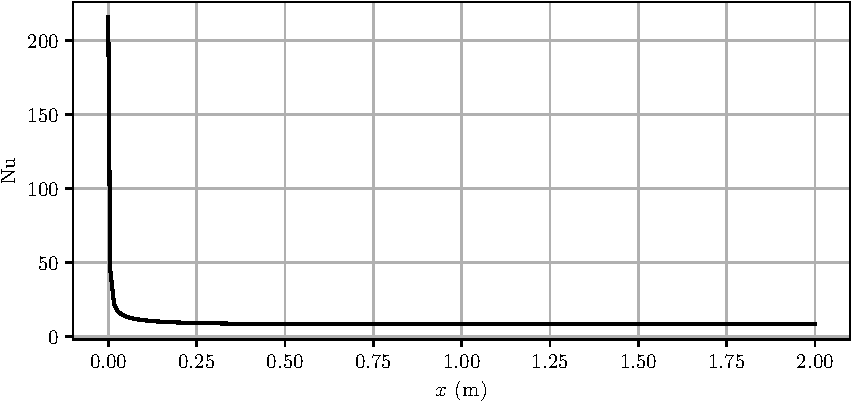
\includegraphics[width=0.75\linewidth]{../results/Nu}
	\caption{The Nusselt number plotted as a function of stream-wise distance for the 180 $\times$ 54 grid.}
	\label{fig:Nu}
\end{figure}

\section*{Code listing}

For the implementation, we have the following files:
\begin{itemize}
	\item \texttt{Makefile} -- Allows for compiling the c++ project with \texttt{make}.
	\item \texttt{hwk4.cpp} -- Contains the \texttt{main()} function that is required by C that runs the cases requested in this problem set.
	\item \texttt{Problem.h} -- Contains the header for the \texttt{Problem} class which is the main driver for a \texttt{Flow2D::Problem}.
	\item \texttt{Variable.h} -- Contains the \texttt{Flow2D::Variable} class, which is a storage container for a single variable (i.e., $u$).
	\item \texttt{Problem.cpp} -- Contains the \texttt{run()} functions that executes a \texttt{Problem}.
	\item \texttt{Problem\_coefficients.cpp} -- Contains the functions for solving coefficients in a \texttt{Problem}.
	\item \texttt{Problem\_corrections.cpp} -- Contains the functions for correcting solutions in a \texttt{Problem}.
	\item \texttt{Problem\_residuals.cpp} -- Contains the functions for computing residuals in a \texttt{Problem}.
	\item \texttt{Problem\_solvers.cpp} -- Contains the functions for sweeping and solving in a \texttt{Problem}.
	\item \texttt{Matrix.h} -- Contains the \texttt{Matrix} class which provides storage for a matrix with various standard matrix operations.
	\item \texttt{TriDiagonal.h} -- Contains the \texttt{TriDiagonal} class which provides storage for a tri-diagonal matrix including the TDMA solver found in the member function \texttt{solveTDMA()}.
	\item \texttt{Vector.h} -- Contains the \texttt{Vector} class for one-dimensional vector storage.
	\item \texttt{postprocess.py} - Produces the plots and tables in this report.
\end{itemize}

\subsection*{Makefile}
\inputminted[fontsize=\scriptsize]{Makefile}{../Makefile}

\subsection*{hwk5.cpp}
\inputminted[fontsize=\scriptsize]{c++}{../hwk5.cpp}

\newpage
\subsection*{Problem.h}
\inputminted[fontsize=\scriptsize]{c++}{../Problem.h}

\newpage
\subsection*{Variable.h}
\inputminted[fontsize=\scriptsize]{c++}{../Variable.h}

\newpage
\subsection*{Problem.cpp}
\inputminted[fontsize=\scriptsize]{c++}{../Problem.cpp}

\newpage
\subsection*{Problem\_coefficients.cpp}
\inputminted[fontsize=\scriptsize]{c++}{../Problem_coefficients.cpp}

\newpage
\subsection*{Problem\_corrections.cpp}
\inputminted[fontsize=\scriptsize]{c++}{../Problem_corrections.cpp}

\newpage
\subsection*{Problem\_residuals.cpp}
\inputminted[fontsize=\scriptsize]{c++}{../Problem_residuals.cpp}

\newpage
\subsection*{Problem\_solvers.cpp}
\inputminted[fontsize=\scriptsize]{c++}{../Problem_solvers.cpp}

\newpage
\subsection*{Matrix.h}
\inputminted[fontsize=\scriptsize]{c++}{../Matrix.h}

\newpage
\subsection*{TriDiagonal.h}
\inputminted[fontsize=\scriptsize]{c++}{../TriDiagonal.h}

\newpage
\subsection*{Vector.h}
\inputminted[fontsize=\scriptsize]{c++}{../Vector.h}

\newpage
\subsection*{postprocess.py}
\inputminted[fontsize=\scriptsize]{python}{../postprocess.py}

\end{document}
